\documentclass[a4paper]{article}
\usepackage{amsmath}
\usepackage{amssymb}
\usepackage{geometry}
\usepackage{enumerate}
\usepackage{natbib}
\usepackage{float}%稳定图片位置
\usepackage{graphicx,subfig}%画图
\usepackage{caption}
\usepackage[english]{babel}
\usepackage{indentfirst}%缩进
\usepackage{enumerate}%加序号
\usepackage{multirow}%合并行
\usepackage{hyperref}
\usepackage{tikz}
\hypersetup{hypertex=true, colorlinks=true, linkcolor=black, anchorcolor=black, citecolor=black}
\title{\Large \textbf{VG441 Problem Set 3}\\
\author{\textbf{Pan, Chongdan ID:516370910121}\\
}
}
\begin{document}
\maketitle
\section{Problem 1}
\quad 
The problem can be consider as a MILP in the following ways:
$$\min \sum_{i=1}^{m}s_i$$
\\s.t.
$$s_i=\{0, 1\},\forall i=0,1\cdots m$$
\begin{center}
    \[x_{ij}=\begin{cases}
        1 & e_j\in S_i\\
        0 & e_j\notin S_i
    \end{cases}\]
\end{center}
$$y_j=\max\{s_1x_{1j},s_2x_{2j}\cdots s_ix_{ij} \}=1,\forall j=0,1\cdots n$$
$i$ is the number of sets, $s_i$ represents whether we select it, $s_i=1$ if we select the $i_{th}$ set, otherwise 0
$j$ is the number of elements, and $x_{ij}$ represents whether $e_j\in S_i$, if it's covered by $S_i$, then 1, otherwise 1. $y_j$ represents whether the $j_{th}$ element $e_j$ is covered by our selection, it's 1 if covered, otherwise 0. Hence all $y_j$ should be 1 because we want to cover all elements.
\par Our objective is to minimize the sum of $x_{s_i}$, which represents the number of set selected.
\begin{figure}[H]
    \centering
    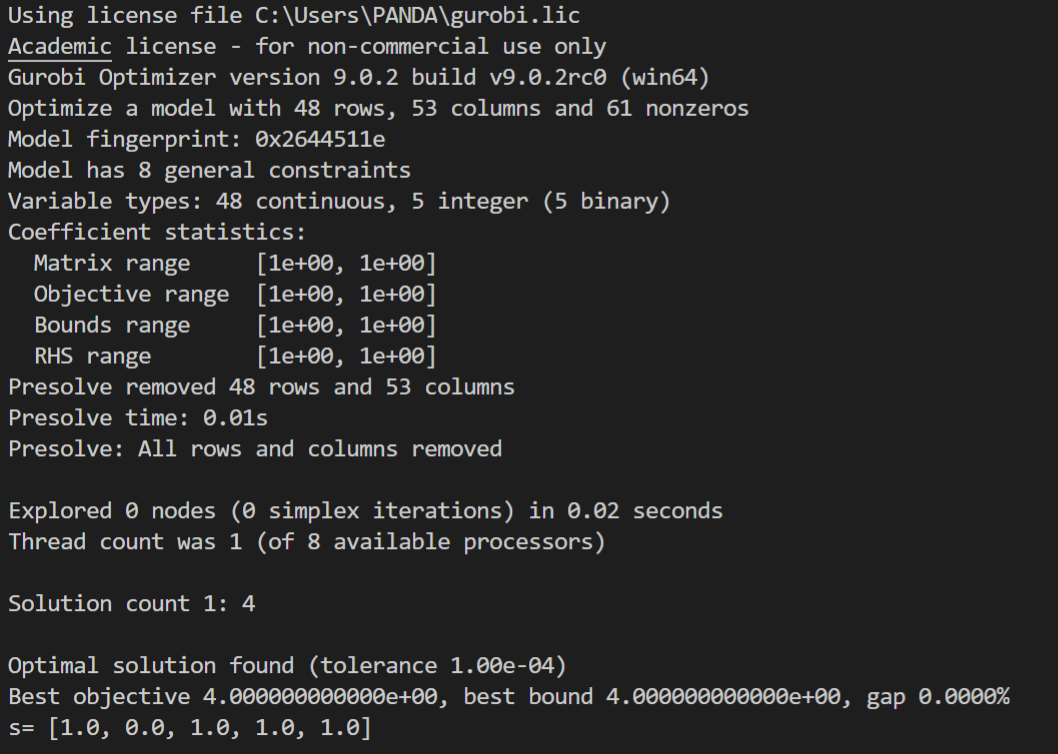
\includegraphics[scale=0.5]{P1.png}
    \caption{Result from Gurobi}
\end{figure}
\par According to solution from Gurobi, we get that we should choose $S_1,S_3,S_4,S_5$ so that all elements are covered, the minimize number of set is 4.
\section{Problem 2}
For a Fractional Knapsack problem, the object is:
$$\max\sum_{i=1}^{n}v_i x_i$$
\\s.t.
$$\sum_{i=1}^{n}s_i x_i\leq B$$
$$0\leq x_i\leq 1,\forall i$$
\\According to greedy algorithm, we need to create a new list  $[\frac{v_1}{s_1}\geq \frac{v_2}{s_2}\cdots\geq \frac{v_i}{x_i}]$, and the solution is $x=[1, 1\cdots 1,x_k,0\cdots,0]$ such that $\sum_{i=1}^{k-1}s_i + x_ks_k=B$, then the value of object function is $\sum_{i=1}^{k-1}v_i + x_kv_k$.
\\Assume we can have a better solution by taking items with total $\bigtriangleup s$ from the greedy algorithm solutions and add items with total $\bigtriangleup s'$ to it. $\bigtriangleup s\geq\bigtriangleup s'\geq 0$ because $\sum_{i=1}^k s_i\leq B$
\\The value we take with $\bigtriangleup s$ is bounded by $\frac{v_k}{s_k}\bigtriangleup s\leq\bigtriangleup v\leq \frac{v_1}{s_1}\bigtriangleup s$
\\The value we can add with $\bigtriangleup s'$ is also bounded by $0\leq\bigtriangleup v'\leq \frac{v_k}{s_k}\bigtriangleup s'\leq \frac{v_k}{s_k}\bigtriangleup s$
\\Hence the net value we can add $\bigtriangleup v'-\bigtriangleup v\leq\frac{v_k}{s_k}\bigtriangleup s-\frac{v_k}{s_k}\bigtriangleup s=0$
\\Therefore, we can't add any value to the solution from greedy algorithm anymore, and it gives the optimal solution.
\newpage
\section*{Python Code}
\begin{verbatim}
    import numpy as np
    import pandas as pd
    from gurobipy import *
    import matplotlib.pyplot as plt

    # 读取数据
    data = pd.DataFrame(pd.read_csv('D:\PANDA\Study\VG441\Homework\Problem Set 3\Data.csv'))
    data = data.iloc[:, 1:]
    m = data.shape[0]
    n = data.shape[1]
    # 初始化数据
    X = []
    t = []
    for i in range(m): X.append(list(data.loc[i])) 
    WW = Model()
    s = WW.addVars(m, vtype=GRB.BINARY, name="set_if_selected") # m sets
    y = WW.addVars(n, name="element_if_covered") # n elements covered
    WW.setObjective(quicksum(s), GRB.MINIMIZE)
    for i in range(0, m):
        t.append(WW.addVars(n))
        WW.addConstrs(t[i][j] == s[i]*X[i][j] for j in range(n))
    WW.addConstrs(y[j] == max_(t[i][j] for i in range(m)) for j in range(n))
    WW.addConstrs(y[j] == 1 for j in range(n))
    WW.optimize()
    print('s=',WW.getAttr('X',s).values())
\end{verbatim}
\end{document}